\documentclass{article}

\usepackage{geometry}
\usepackage{amsmath}
\usepackage{graphicx}
\usepackage{listings}
\usepackage{hyperref}
\usepackage{multicol}
\usepackage{fancyhdr}
\pagestyle{fancy}
\hypersetup{ colorlinks=true, linkcolor=black, filecolor=magenta, urlcolor=cyan}
\geometry{ a4paper, total={170mm,257mm}, top=20mm, right=20mm, bottom=20mm, left=20mm}
\setlength{\parindent}{0pt}
\setlength{\parskip}{1em}
\renewcommand{\headrulewidth}{0pt}
\lhead{Competitive Programming - Arkavidia V}
\fancyfoot[CE,CO]{\thepage}
\lstset{
    basicstyle=\ttfamily\small,
    columns=fixed,
    extendedchars=true,
    breaklines=true,
    tabsize=2,
    prebreak=\raisebox{0ex}[0ex][0ex]{\ensuremath{\hookleftarrow}},
    frame=none,
    showtabs=false,
    showspaces=false,
    showstringspaces=false,
    prebreak={},
    keywordstyle=\color[rgb]{0.627,0.126,0.941},
    commentstyle=\color[rgb]{0.133,0.545,0.133},
    stringstyle=\color[rgb]{01,0,0},
    captionpos=t,
    escapeinside={(\%}{\%)}
}

\begin{document}

\begin{center}
    \section*{E. Eksplorasi Pola}

    \begin{tabular}{ | c c | }
        \hline
        Batas Waktu  & 1s \\
        Batas Memori & 512MB \\
        \hline
    \end{tabular}
\end{center}

\subsection*{Deskripsi}

Suatu hari, Arvy sedang belajar bermain rubik berukuran $N \times N \times N$.
Ia merepresentasikan jenis putaran yang ia lakukan pada rubik dengan perintah $X_i, x_i, Y_i, y_i, Z_i, z_i$ ($1 \leq i \leq N$) dengan arah rotasi seperti pada gambar.
Sebagai contoh, $X_1$ akan memutar rubik searah dengan panah warna hijau, $y_2$ akan memutar rubik searah dengan panah warna ungu, $Z_2$ akan memutar rubik searah dengan panah warna hitam.
Perintah $Z_2, z_1$ akan mengubah rubik pada bagian kiri menjadi rubik pada bagian kanan.

\begin{center}
    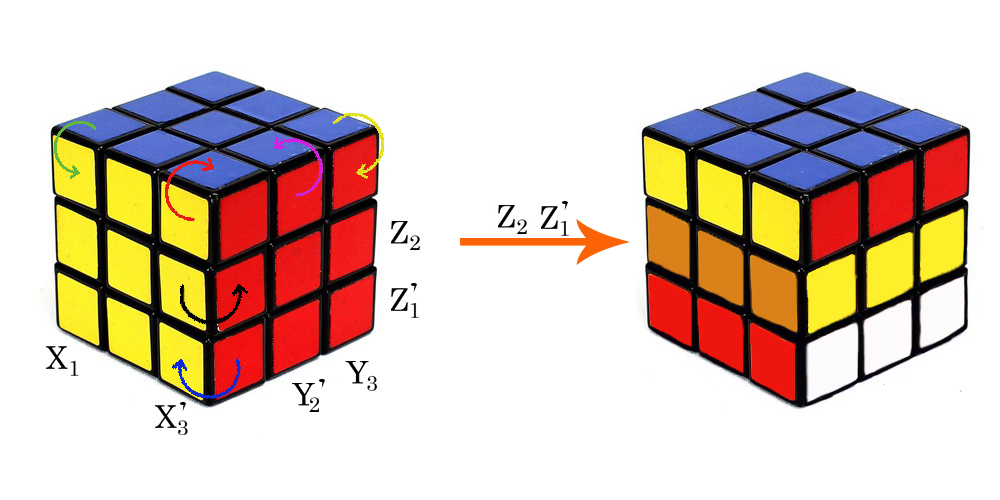
\includegraphics[width=250px]{rubic}
\end{center}

Ia menyadari ada hal yang unik dari putaran ini.
Pertama, Arvy menuliskan beberapa perintah pemutaran rubik.
Kemudian, ia melakukan perintah yang ia tulis tadi berulang-ulang dan ternyata rubik dapat kembali ke pola semula.
Arvy penasaran berapa kali ia harus mengulang perintah yang sama agar rubik kembali ke pola semula.

\subsection*{Format Masukan}

Baris pertama terdiri dari satu bilangan bulat positif $T$ ($1 \leq T \leq 10$), menyatakan banyaknya kasus uji.
Untuk tiap kasus uji, akan terdapat $M + 1$ baris.

Baris pertama terdiri dari bilangan bulat $N$ ($2 \leq N \leq 20$) menyatakan ukuran rubik dan $M$ ($1 \leq M \leq 100.000$) menyatakan panjang perintah.
$M$ baris berikutnya berisikan sebuah perintah, masing-masing dengan format \lstinline{C i}.
\lstinline{C} merupakan \lstinline{X}, \lstinline{x}, \lstinline{Y}, \lstinline{y}, \lstinline{Z}, atau \lstinline{z}, menyatakan dimensi dan arah perputaran.
\lstinline{i} menyatakan bagian yang diputar ($1 \leq i \leq N$).

\subsection*{Format Keluaran}

Untuk tiap kasus uji, tuliskan dalam satu baris, banyaknya pengulangan perintah yang sama (lebih dari 0) agar rubik kembali ke pola semula.
\\

\begin{multicols}{2}
\subsection*{Contoh Masukan}
\begin{lstlisting}
2
3 2
Y 2
y 1
2 3
x 2
Y 1
z 1
\end{lstlisting}
\columnbreak
\subsection*{Contoh Keluaran}
\begin{lstlisting}
4
\end{lstlisting}
\vfill
\null
\end{multicols}

\subsection*{Penjelasan}
Pada kasus uji pertama, cukup dengan menjalankan rangkaian perintah sebanyak 4 kali, rubik akan kembali seperti semula, seperti pada gambar di bawah:
\begin{center}
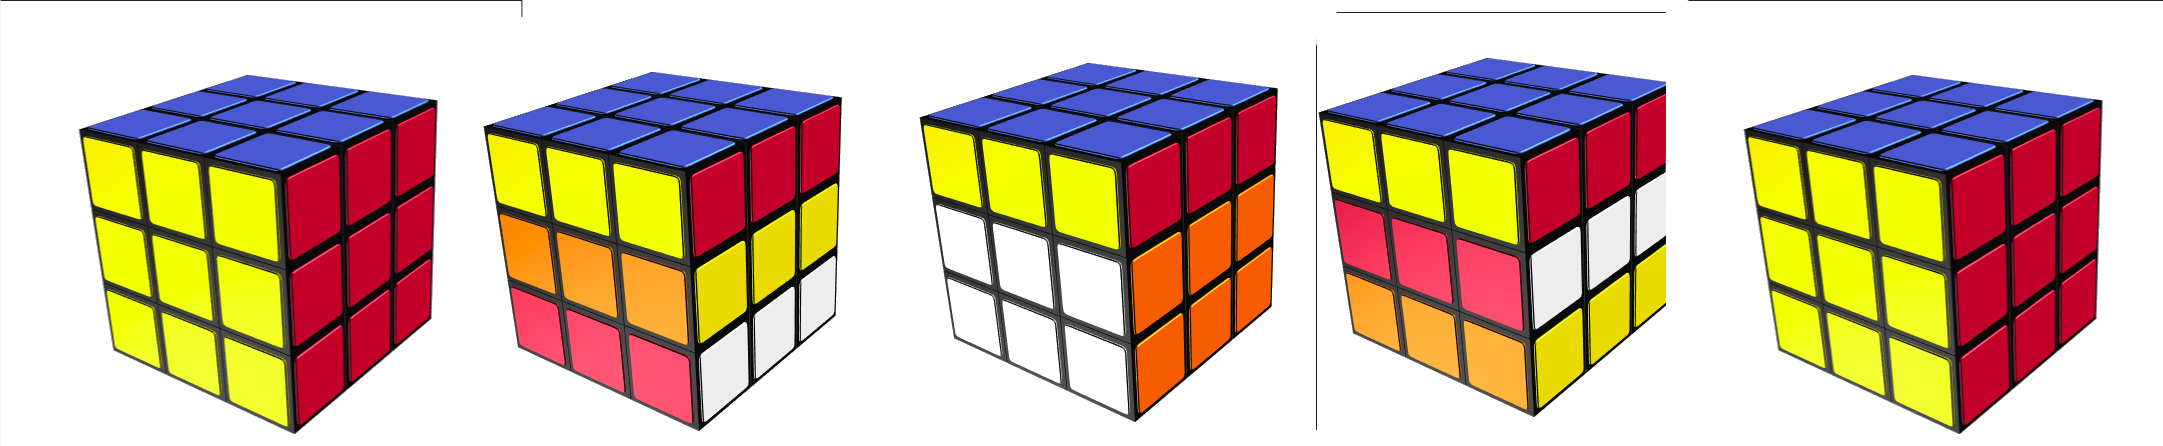
\includegraphics[width=400px]{sample-1}
\end{center}
Pada kasus uji kedua, cukup dengan menjalankan rangkaian perintah sebanyak 30 kali, rubik akan kembali seperti semula, seperti pada gambar di bawah:
\begin{center}
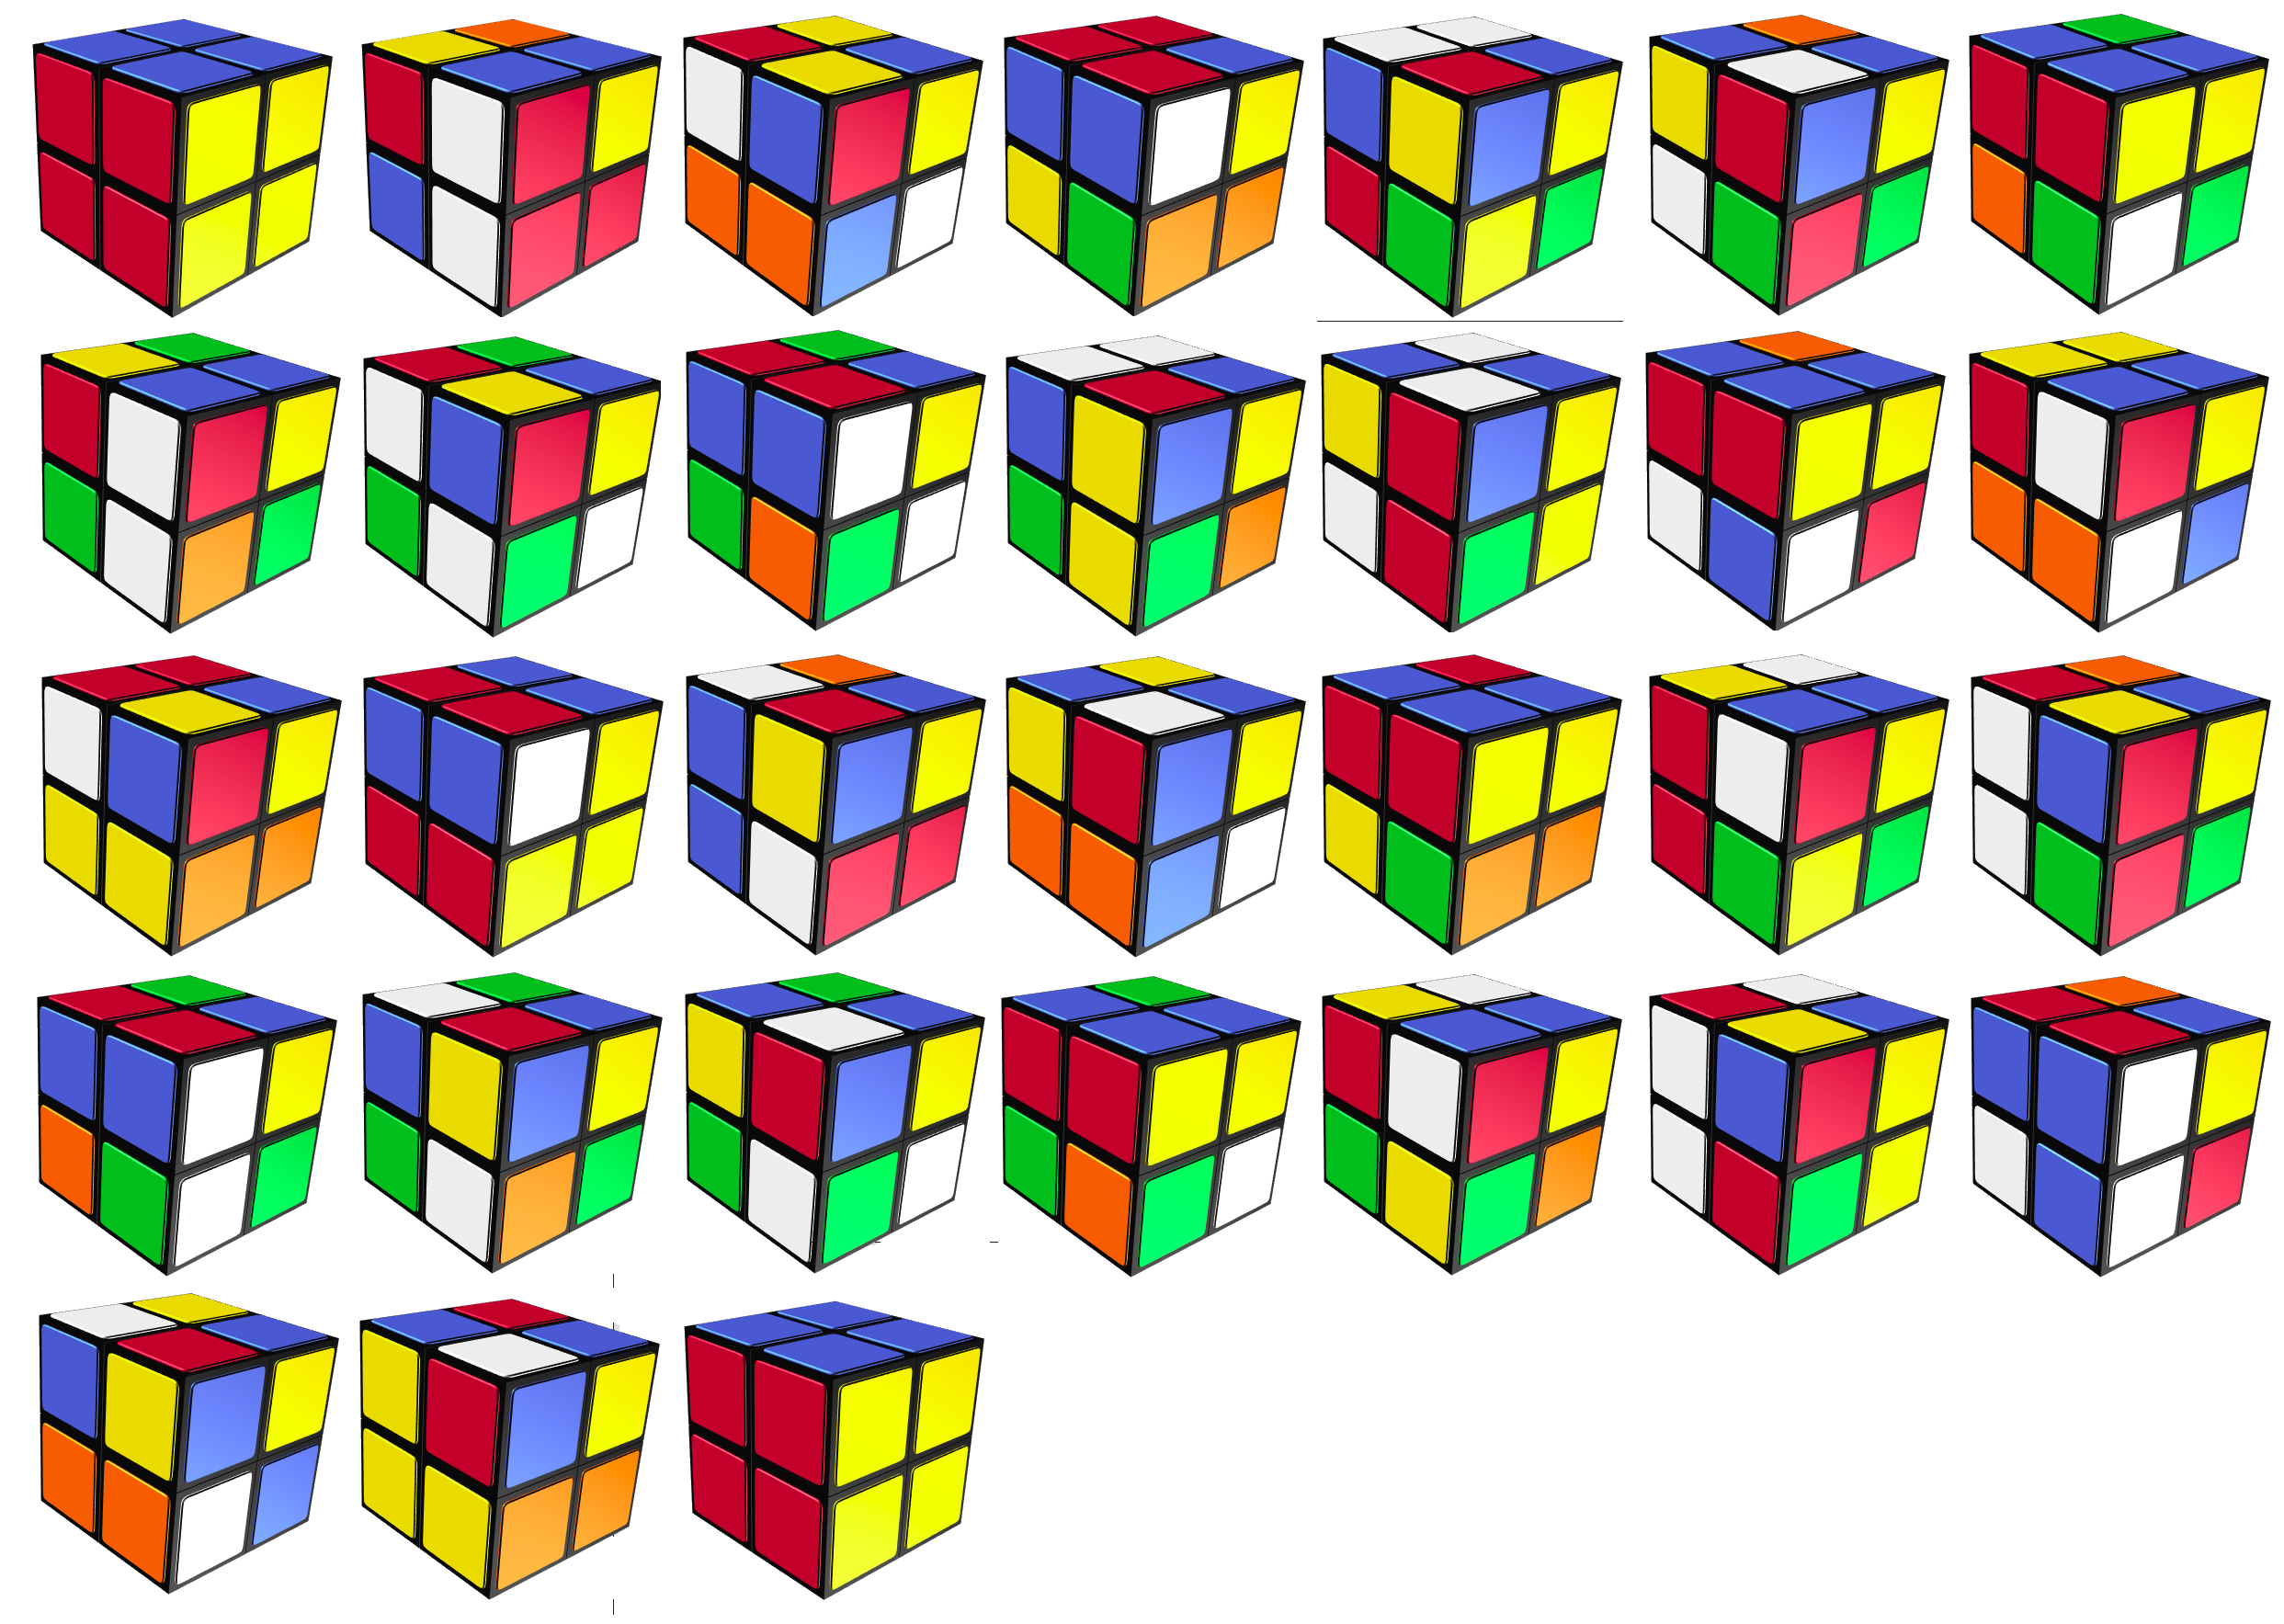
\includegraphics[width=450px]{sample-2}
\end{center}
\pagebreak

\end{document}